\chapter{General Introduction}

\section{The ocean, phytoplankton and why it matters}
The complexity of the ocean and its vast ecosystems has fascinated scientists to this day and most likely will continue to do so far into the future. Myriad life forms are embedded in a matrix so far removed from our mostly dry existence on top the earth’s crust. In the ocean, life moves in dilution, and the equivalents of forests and grasslands are hard to spot unless the concentration of tiny phytoplankton is so large, that deep blue turns into a milky green.

The term phytoplankton refers to microscopic marine photosynthetic organisms. These microorganisms form the basis of the oceanic food web and are primary producers of planetary scale, contributing roughly half of the oxygen in our atmosphere through photosynthesis \citep{Field2009}. Phytoplankton consists of mostly single-celled organisms, prokaryotes and eukaryotes from a highly diverse evolutionary background \citep{Falkowski2004a}. This large genetic diversity is accompanied by a remarkable range of survival strategies, biogeochemical roles, shapes and sizes within the polyphyletic phytoplankton (see Figure \ref{FinkelPhySizeRange} for a size comparison). 
The emergence of such a large range of organisms and the mechanisms sustaining their persistence has been one of the key topics in phytoplankton ecology over the last 50 years. Hutchinson's paradox.X(REF here)X

\begin{figure}
\centering
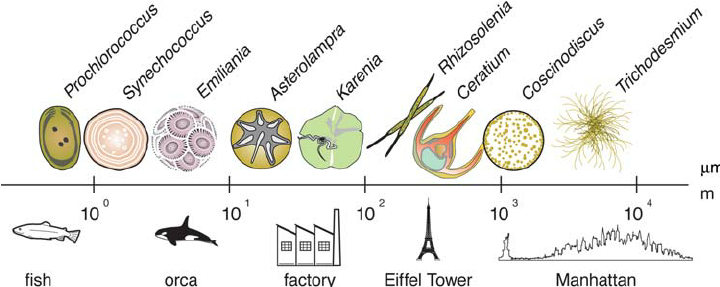
\includegraphics[trim = 0mm 0mm 0mm 0mm, clip, width=.9\linewidth]{./Chp1-Intro/SIZEphytoComparison_FinkelEtAl2010.png}
\caption[Scheme]{\small {"A comparison of the size range (maximum linear dimension) of phytoplankton
relative to macroscopic objects." from \cite{Finkel2010}}}
\label{FinkelPhySizeRange}
\end{figure}

||| also explain MLD in the following paragraph |||

The distribution of phytoplankton is driven by the complex physical forces that govern ocean currents and the chemistry of the bodies of water the move. The key components are macronutrients (e.g. nitrogen \& phosphorus) and micronutrients (e.g. iron \& cobalt) welling up from the deeper ocean or flushed in from continental sources. Wherever there are sufficient nutrients available within the euphotic zone, the depth where photosyntheticaly available radiation (PAR) is 1\% of the surface value, planktonic life begins to thrive. Ecosystems along continental margins provide a particularly productive habitat, with only 10\% of total ocean surface area covered by continental margins, but 10-15\% of marine primary production and more than 40\% of carbon export to the seabed occurring along coastal lines \citep{Yool2001,Muller-Karger2005}.


Phytoplankton growth indirectly feeds a considerable part of earth’s population through fisheries \citep{Stock2017} and even shapes the elemental composition of oceanic water itself \citep{Redfield1958}. 
The biomass produced is mostly consumed by higher trophic levels and either assimilated or excreted. Another large portion experiences natural mortality and viral lysis. Microbial degradation drives remineralization within the euphotic zone, which fuels regenerated production \citep{Eppley1979} [Perhaps put quotation about Microbial Loop here!]. 
A small fraction sinks out of the photic layer as fecal or detrital matter to the deeper ocean and an even smaller fraction reaches the sea floor as sediment ( roughly 1 \%) and remains there over geological times \citep{Honjo2008}. This process has been termed the biological carbon pump. Carbon sequestered this way is removed from the ocean-atmosphere system for potentially millions of years. Given the projected rise of atmospheric CO$_2$ levels, it is of grave importance to understand how changes in the phytoplankton community at the surface, driven by anthropogenic stressors and climate change, will affect the carbon burial potential of oceanic ecosystems. 
Studies have both reported a global declining trend in marine primary production \citep{Boyce2012} and increasing trends in long-term ocean time series \citep{Chavez2011a}. 
In order to answer questions of how phytoplankton will respond to a changing climate it is necessary to look the diverse phytoplankton community in greater detail. 

\section{Characterizing phytoplankton}
From the early days of oceanographic research, scientists have been interested in the microscopic organisms that were floating in samples of sea water. These communities contain many species each and in total there are tens of thousands of species of phytoplankton that inhabit the surface ocean \citep{Engelen2015}. All phytoplankton species use chlorophyll or bacteriochlorophyll to harvest light as the energy source to fix organic carbon, but there is wide variation in virtually all their other properties \citep{Litchman2008}. In addition to the complex community composition, there are many factors affecting measurements of their bulk properties in the ocean, such as the viral and bacterial community and the influence of diverse grazers, all within the complex three-dimensional physical environment that is the ocean. 
Where earlier phytoplankton ecologists focused on identifying individual species, decoding their phylogeny or growing them in controlled lab cultures, recent research is trying to integrate the insights gained from these approaches and quantify the diversity on higher levels of organization in relation to other properties of the ecosystem. The focus has shifted towards trait diversity both within and across species and within and across phytoplankton groups. In order to scientifically describe this perplexing diversity the concepts of trait-based ecology and functional types have been developed \citep{Tilman2001,McGill2006,Violle2007c}.

\begin{figure}
\centering
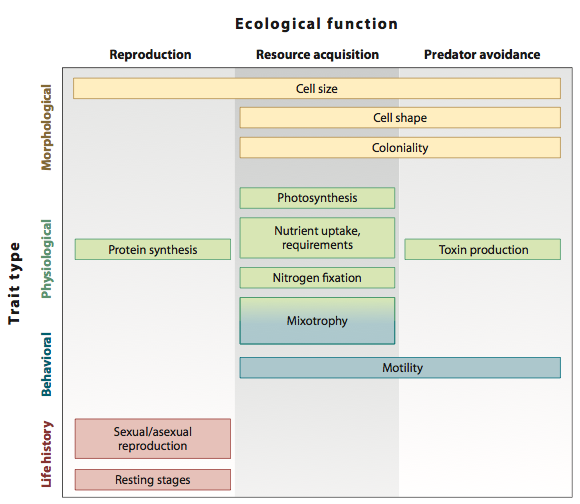
\includegraphics[width=0.7\linewidth]{./Chp1-Intro/Fig_litchman2008.png}
\caption[Scheme]{\small{"A typology of phytoplankton functional traits" from \cite{Litchman2008}}}
\label{PhytoTraits}
\end{figure}

\subsection{Functional types and traits}
In the following I will try to clarify the complementary terms of phytoplankton traits, functional traits, and functional types. 

The trait-based approach to phytoplankton ecology has been growing in popularity. Part of the fascination evoked by this term stems from its origin in evolutionarily theory. Over the last three decades, it has been adopted by ecologists trying to understand communities and ecosystems. In this new context, the concept of traits has been stretched far beyond its original meaning, which can lead to some confusion surrounding the scope of trait-based methods \citep{Violle2007c}. In the simplest definition, a trait is a surrogate of organismal performance. In the ecological context this has been expanded to surrogates for the performance of populations, communities and entire ecosystems. This can include ecophysiological traits, life-history traits, demographic traits or response and effect traits of ecosystems (see Figure \ref{PhytoTraits} for a selection of phytoplankton traits). Theoretically, any property of an organism or ecosystem could be defined as a trait, but ideally a trait should be functional. Functional traits are defined by \cite{Violle2007c} as "morpho-, physio- or phenological traits which impact fitness indirectly via their effects on growth, reproduction and survival". An important facet of the trait-based approach is to describe organismal function via trade-offs between traits. For example when competing for multiple nutrients, phytoplankton species are thought to be constrained by trade-offs in their competitive ability for one over another resource \citep{Tilman1990}. 

Phytoplankton are extremely diverse and the trait based approach lends itself to generalizations, as traits and ecological trade-offs can be defined and explored irrespective of species or taxa boundaries \citep{McGill2006}. However, depending on the study and hypotheses to be tested, it can be very helpful to structure the diversity of organisms into distinct groups. Major taxonomic groups of phytoplankton can be classified based on their ecological or biogeochemical roles within the ecosystem \citep{Iglesias-Rodriguez2002,Flynn2015}. The concept of functional groups is not in contrast to a trait-based ecology of phytoplankton, but can be complementary to it. By broadly sampling relevant traits across phytoplankton groups and species, functional types can be defined by functional traits and trade-offs and therefore extend the trait-based approach by another level of organization \citep{Litchman2007d}. An early example is the work of Ramón Margalef. Margalef used observations of important traits, such as sinking rates and nutrient utilization to build the concept called "Margalef's mandala" to organize phytoplankton functional types (PFTs) on a spectrum of nutrient availability versus turbulence \citep{Margalef1978}. 

The terms functional group and functional type are used interchangeably, with functional groups more often referring to the grouping of species and the functional type describing the group as a whole, often as implemented in computational models. In fact, the simplification of the phytoplankton community into functional types has been widely used for the design and interpretation of computational models that try to recreate or make predictions about the biogeochemical cycling, biogeographic distribution, productivity and other ecosystem functions of phytoplankton \citep{Gregg2003,LeQuere2005}. Biogeochemically defined functional types are most often used, as these functional traits can usually be well defined within an ecosystem model. Typical examples of such functional groups are silicifers, which broadly correspond the phylogenetic group of diatoms, and calcifiers, which are usually represented by coccolithophores. Such functional types are always simplifications of the natural pyhtoplankton diversity. Silicoflagellates create silicified skeletons like diatoms, but are often not explicitly included because they rarely dominate modern phytoplankton assemblages. The choice of which functional groups to include in a model can also be driven by biogeography or analytical considerations concerning the measurement instrumentation used for a particular study \citep{IrwinAndrewJ.Finkel2017b}. 

||||Perhaps small paragraph about functional diversity here?||||
In biodiversity research, the trait-based approach has been readily adopted. It used to be that species diversity (i.e. the number of species) was the most important metric, but now it is functional diversity, which can be described by the variance in the value of a functional trait of the community or ecosystem.

It is important to keep in mind that functional types are often composed of many species with a possibly large variance in trait values. Recent research is trying to understand the effects of diversity within functional types and within species \citep{Violle2012,Violle2017a,DesRoches2018}.




\section{Modeling phytoplankton communities}
Given the complexity of the ocean ecosystem, it is necessary to aggregate our knowledge of the many smaller parts into comprehensive ecological models in order to test mechanistic hypotheses and investigate their full-scale implications. 

Computational models of phytoplankton growth have been developed since the 1940s and have greatly increased in sophistication and complexity since then, co-evolving with the rise in computational resources \citep{Gentleman2002a}. Phytoplankton modelling started with formulations based on the Lotka-Volterra equations of predator-prey dynamics \citep{Fleming1939}. From these relatively simple descriptions of the populations, models evolved to describe the oceanic physical environment in ecosystem models including multiple trophic levels. Originally developed by John Steele with a model ocean split in two layers, the nutrient-phytoplankton-zooplankton (NPZ) and nutrient-phytoplankton-zooplankton-detritus (NPZD) models succeeded in reproducing the basic bloom dynamics observed in the temperate ocean \citep{Steele1958,Evans1988,Fasham1990a}. Further developments have been in more exact physiological descriptions of phytoplankton based in cellular metabolism and energy allocation \citep{Geider1997} and both simple and more complicated ecosystem formulations driven by local and global 3D circulation models \citep{Lacroix2007, Hirata2013}.

However, in their simplified approach, these models unavoidably limit the characterization of a diverse phytoplankton community \citep{Bruggeman2009}. These plankton ecosystem models are typically highly aggregated, such that a single variable determines the response of a diverse assemblage of phytoplankton species \citep{Franks2009}. Implementing a meaningful treatment of biodiversity in ecological models is a key challenge in the field of phytoplankton modeling \citep{Queiros2015}. The most apparent way of implementing this within the framework of established NPZD models is to include multiple equations and state variables for different phytoplankton functional types \citep{LeQuere2005}. For every group that fulfills a distinct ecosystem function, a new set of parameters has to be added, which complicates the model structure and increases computational costs. This somewhat intuitive approach, however, does lead to problems. First and foremost, this is the lack and inherent uncertainty of data from field and culture experiments to constrain functional types. This again leads to the difficulty of validating the model output in light of insufficient information, leading multiple authors to criticize the PFT modeling approach as attempting to "run before we can walk" particularly when used for extrapolating into the future \citep{Anderson2005,Shimoda2016}. 

The current scientific discussion can seem intimidating to an early career scientist, as both the most obvious future directions of ecosystem model design as exemplified by PFT models, as well as the very foundation of traditional NPZD models has come under scrutiny. Nowhere is this more apparent as with the formulation of nutrient uptake dynamics, which is traditionally defined by Monod kinetics that are based on the equations for Michealis-Menten enzyme kinetics. (Monod reference here)

ALSO: current modeling paradigms are discussed quite critically in the literature, in particular the Monod kinetics and also the lack of any adaptive mechanisms in these model \citep{Smith2014}
A bit earlier, but similar direction: \citep{Flynn2010}
and more recent, but focused on Monod: \citep{Hellweger2017a}

However, there are also examples of modeling approaches that show a way forward. To name an alternative to the modeling paradigm discussed so far, there is individual based modeling (IBM). In IBM the phytoplankton are explicitly represented as individual agents, allowing for a diverse and spatially interactive phytoplankton community \citep{Hellweger2009}. The computational cost and structural complexity of this approach however does not yet lend itself well to studies of large-scale or even global ecosystems. 

Another approach which lends itself very well to just such studies is to extend traditional NPZD models via moment-based estimation of aggregate properties \citep{Merico2009}. A specific implementation of this is the PhytoSFDM model developed by \citet{Acevedo-Trejos2016}. Instead of modeling multiple size-classes of phytoplankton explicitly, the community is described with a single equation that describes not only the biomass, but also the mean size, and size variance. Size is used as a master trait, with size variance as a proxy for functional diversity. Trade-offs related to nutrient uptake, grazing and sinking structure the phytoplankton community along the size spectrum as driven by the physical forcing. The model was used to investigate latitudinal diversity gradients in the Atlantic Ocean \citep{Acevedo-Trejos2018}. One point of criticism for this approach is that the size distribution is fixed to the shape of a skewed log-normal distribution, not allowing for the emergence of other, for example multi-modal, distributions that have been observed in natural phytoplankton communities. 
 
 And the aggregate moment based models such as PhytoSFDM! (TRAIT-BASED-APPROACH)

And the DARWIN model, including Ben Wards adaptation, including multiple PFTS with a trait-based parametrisation for each functional type based on the organismal size range! (TRAIT-BASED-APPROACH)


A simple example of a trait-based description of phytoplankton succession is scaling the maximal nutrient acquisition rate and the respective affinity with cell size. A trade-off would emerge between different size classes, allowing for a modeled succession along gradients of nutrient depletion. One example of a very similar approach is the PhytoSFDM model developed by Acevedo-Trejos and colleagues (XAcevedo‐Trejos et al. 2013, Acevedo-Trejos et al. 2015X). In their approach, the trait-based modeling of phytoplankton is even further simplified, by describing an entire community as a size- distribution with a mean value and a variance, instead of modeling all the different size classes explicitly. This moment-based structure further simplifies the mathematical basis of the model, and leads to much faster processing times and less uncertainty in parameter estimation.



"need to identify the basic uncertainties and see if there is a way to discuss them scientifically
"Michaelis Menten kinetics are really outdated.. and i suppose using them in a trait-based modelling approach is questionable just the same





XXX

XXX

XXX

XXX. 

XXX

XXX

ALWAYS NEED A GOOD BASIS IN DATA TO VALIDATE MODELS AND HYPOTHESES

\section{The Cariaco basin \& the CARIACO time series}

A coastal tropical ecosystem, continental margins important site of marine PP


"The Cariaco Basin, located off the coast of Venezuela, has been the site of high frequency water column sampling for marine biogeochemical and ecological observations since 1995. The observations were collected as part of the Cariaco Ocean Time-Series Program (Muller-Karger et al., 2001; Thunell et al., 2007). 

XXXX

In addition to the recent importance of the cariaco basin as the site of an important paleo-oceanographic time sereis, the Cariaco basin has served as a natureal laboratory for biogeochemists for over 50 years. This basin has been key in constructiong stoichiometric models of organic matter remineralization (Redfield et al 1963 and Richards 1975!), developing residence time and box models, and numerous other studies.

\begin{figure}
\centering
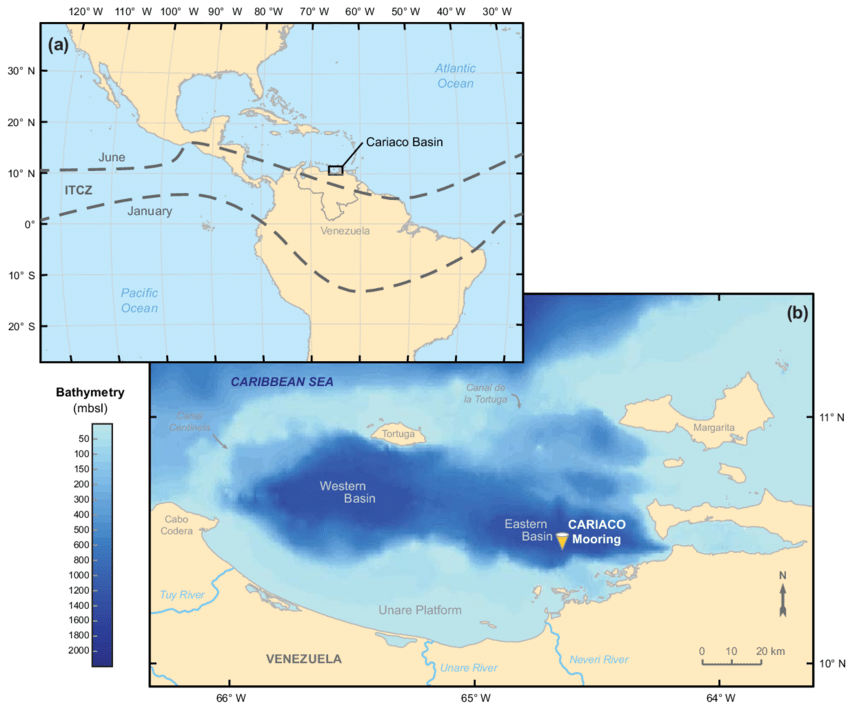
\includegraphics[trim = 0mm 0mm 0mm 0mm, clip, width=1.\linewidth]{./Chp1-Intro/CARIACObasinMAP_Bringueetal2018.png}
\caption[Scheme]{\small {"Study area. A. Location of the Cariaco Basin off the Venezuelan coast in the southern Caribbean Sea, with January and June positions of the Intertropical Convergence Zone (ITCZ). B. Location of the CARIACO station in the eastern sub-basin, general bathymetry and local rivers emptying in the basin (bathymetric data from GEBCO\_08 Grid)" from \cite{Bringue2019}}}
\label{CARIACO-map}
\end{figure}

XXXX

XXX

THEN TALK ABOUT THE COLLABorDATASHARE WITH JPINCKNEY AND CBENITEZNELSON, and how this allows an even deeper look at the biomass dynamics


\section{Aims of the proposed PhD project}
"The general goal of my Ph.D. project is to study the processes that structure the phytoplankton community in contrasting environmental regions of the Atlantic Ocean, using a trait-based modelling perspective. The specific aims during the course of the project are to:

\begin{itemize}
\item MANUSCRIPT 1 "Understanding Shifts in CARIACO"
\item MANUSCRIPT 2 "technical paper" - Geoscientific Model development
\item MANUSCRIPT 3 "BDEF in CARIACO"
\end{itemize}
